\section{Neural Networks}

In this short section, we briefly describe artificial neural networks and their various types relevant to this thesis. However, our assumption is that the reader is sufficiently equipped with the knowledge regarding deep machine learning, and thus, for the sake of keeping this document as short as possible, we will omit detailed elaboration.

% ########################################
\subsection{Artificial Neural Networks}
\label{ssec:ArtificialNeuralNetworks}

Artificial neural networks (or just neural networks for short) are computing systems that are inspired by, but not identical to, biological neural networks that constitute animal brains. Such systems essentially \emph{learn} to perform tasks by considering multiple samples, generally without being programmed with task-specific rules. Within recent decades, under the influence of constantly growing computational power and our data collecting and data processing capabilities, this technology has acquired a status of paramount importance when solving a problem using machine learning. They are a quintessential deep learning model. Artificial neural networks are also known in the literature as the multilayer perceptron~\cite{Rosenblatt1958ThePA}, feedforward neural networks or deep feedforward neural networks~\cite{Goodfellow-et-al-2016}.

In mathematical terms, the goal of a neural network is to approximate some unknown function $f$. For instance, when considering a classifier, the transformation $y = \func{f}{\vx}$  maps the given input $\vx$ to a category $y$. Such a network, therefore, defines a mapping and learns the value of the parameters that result in the best function approximation~\cite{Goodfellow-et-al-2016}.

The name \emph{feedforward} is derived from the fact that the information flows through the function being evaluated from $\vx$, through the intermediate computations, and finally to the output $\vy$. Moreover, the feedforward neural networks are called networks since they are typically represented as a composition of multiple different functions. Such a model can be described with a directed acyclic graph denoting the sequential composition of several functions. More concretely, we might have three functions $\suprbrackets{f}{1}$, $\suprbrackets{f}{2}$ and $\suprbrackets{f}{3}$, forming a chain, $\func{f}{\vx} = \func{\suprbrackets{f}{3}}{\func{\suprbrackets{f}{2}}{\func{\suprbrackets{f}{1}}{\vx}}}$. These chain structures are the most commonly used structures in neural network models~\cite{Goodfellow-et-al-2016} (see Fig.~\ref{fig:TypicalFCNArchitecture}). Deep machine learning consists of multiple such layers of neurons stacked onto each other that are trained using the \emph{backpropagation} algorithm~\cite{rumelhart:errorpropnonote}. Our work will rely heavily upon the aforementioned deep neural networks, especially convolutional neural networks, discussed next.

\begin{figure}[t]
    \centerline{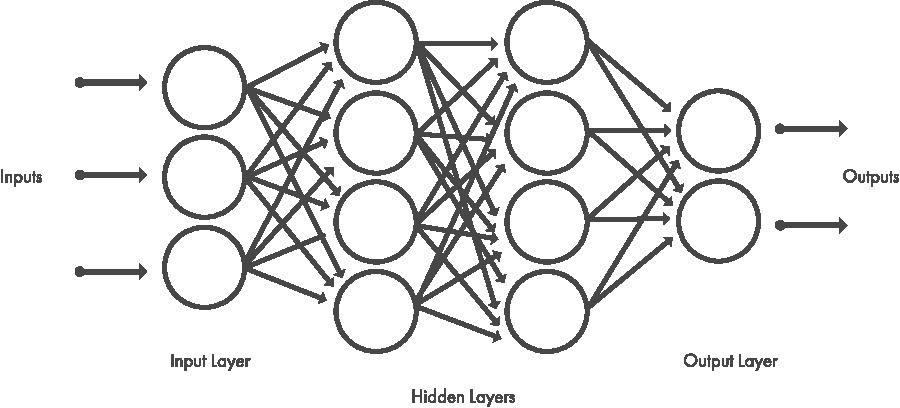
\includegraphics[width=0.8\linewidth]{figures/theoretical_foundations/typical_fcn_architecture.pdf}}
    \caption[A typical FC architecture]{An illustration of a typical fully connected neural network. \externalsrc{\cite{typicalfcnarchitecture}}}
    \label{fig:TypicalFCNArchitecture}
\end{figure}

% ########################################
\subsection{Convolutional Neural Networks}
\label{ssec:ConvolutionalNeuralNetworks}

This type of neural networks has gained popularity in the computer vision community thanks to a never-seen-before performance on image classification task~\cite{Krizhevsky2012}. This machine learning algorithm processes images or other high dimensional, grid-like input and then learns the importance (weights and biases) of various aspects of the input data. Even though \glspl{cnn} can handle $1D$ time series data and be a counterpart to \glspl{rnn}~\cite{franoischollet2017learning}, our primary focus is to process $3D$ tensors. Simply put, convolutional networks are artificial neural networks that use in at least one of their layers the convolution operation instead of a general matrix multiplication~\cite{Goodfellow-et-al-2016} (\cref{fig:TypicalCNNArchitecture}).

The successful ability of these networks to capture spatial and temporal properties via learned convolutional filters is the fundamental principle. Let $f$ and $g$ be functions. Then, the operation of convolution denoted by $\star$ produces a third function, as a result of the following computation (demonstrating the commutativity property, too)~\cite{Goodfellow-et-al-2016}:

\begin{equation}
    \label{eq:ConvolutionContinuous}
    \func{\rbrackets{f \star g}}{t} =
    \int_{-\infty}^{\infty}
    \func{f}{\tau}
    \func{g}{t - \tau}
    d\tau =
    \int_{-\infty}^{\infty}
    \func{f}{t -\tau}
    \func{g}{\tau}
    d\tau.
\end{equation}

\noindent In this setting, $f$ will be the input, and $g$ be the kernel. The output of this operation is a feature map. During the training, the aim is to learn the weights of the kernel matrix (similar to general artificial neural networks) that produces a feature map based on which the model can solve the given task according to some objective function.

Let $I$ be a two-dimensional input image and $K$ be a two-dimensional kernel. Then, for a given position $\rbrackets{i, j}$ in the input image $I$, the convolution can be written in its discrete form as

\begin{equation}
    \label{eq:ConvolutionDiscrete}
    \func{\rbrackets{f \star g}}{i, j} =
    \sum_{m}
    \sum_{n}
    \func{I}{m, n}
    \func{K}{i - m, j - n}.
\end{equation}

\noindent Nonetheless, many machine learning libraries implement the cross-correlation operation, not the convolution operation by its strict definition. This operation is the same except for the fact that the kernel is not flipped, thus the commutative property is not preserved, which is not demanded in neural networks. In that case, the result of the cross-correlation is given by~\cite{Goodfellow-et-al-2016}

\begin{equation}
    \label{eq:CrossCorrelation}
    \func{\rbrackets{f \star g}}{i, j} =
    \sum_{m}
    \sum_{n}
    \func{I}{i + m, j + n}
    \func{K}{m, n}.
\end{equation}

An indispensable outcome of \glspl{cnn} is the ability to capture hierarchical relations. Layers placed near the input to the model capture low-level features such as edges, colors, gradient orientations, and so on. On the other hand, layers placed further, deeper in the model, highlight semantic, abstract features that are specific to the task at hand. We will refer to this fact many times in our work since object trackers need to accurately discriminate between the foreground and background as well as properly generalize. The exploitation of these qualities of convolutional layers will be demonstrated in the \cref{sec:VisualObjectTracking}.

Another prominent use case of \glspl{cnn} is \emph{transfer learning}, where a pretrained model is adopted for a new task, utilizing the already learned features. These pretrained models may come in various flavors, but typical ones are pretrained for an image classification task using the ImageNet dataset~\cite{JiaDeng2009}. The reasoning is that visual features such as edges and contours are vital to general object recognition tasks, hence it is not needed to learn coarse, rudimentary, low-level features from scratch all the time. Our work will certainly require the \emph{transfer learning,} maybe even additional \emph{fine-tuning} of the pretrained model of choice.

\begin{figure}[t]
    \centerline{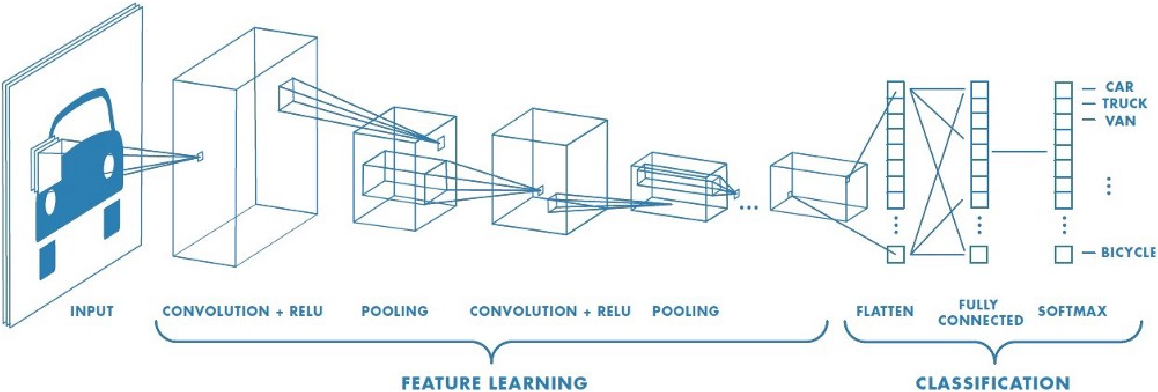
\includegraphics[width=0.9\linewidth]{figures/theoretical_foundations/typical_cnn_architecture.pdf}}
    \caption[A typical CNN architecture]{An illustration of a typical convolutional neural network architecture for a quintessential classification task. An image of a car is fed into the model that extracts visual features that are subsequently processed by the fully connected layers resulting in the probability distribution over target classes. \externalsrc{\cite{typicalcnnarchitecture}}}
    \label{fig:TypicalCNNArchitecture}
\end{figure}
